\begin{figure}[H]
	\centering
	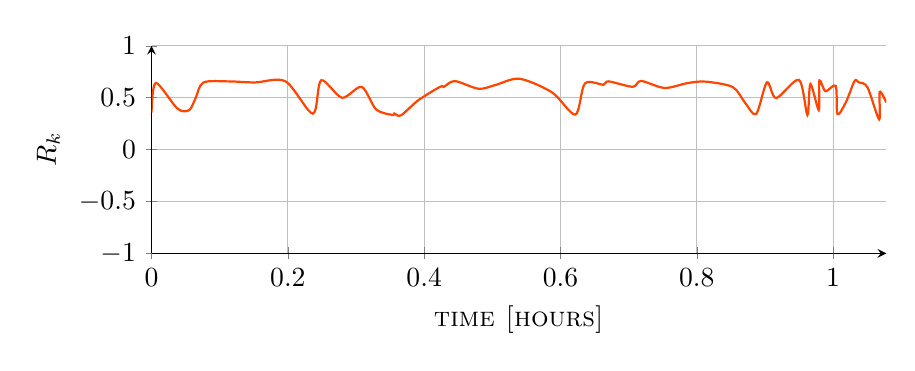
\begin{tikzpicture}
		\begin{axis}[xlabel=\textsc{time [hours]}, ylabel=\textsc{$R_k$}, axis lines=left, grid=major, width=0.9\linewidth, height=12em, ymax=1, ymin=-1]
			\addplot +[mark=none, OrangeRed, thick, smooth] table {
				0.0 0.35546617052879226
				0.006223611111111111 0.6423156409962552
				0.03802861111111111 0.3948780449789209
				0.05518527777777778 0.3799493280869101
				0.06458861111111111 0.4949206401970054
				0.07599277777777778 0.6461311764773638
				0.112955 0.6571725336164813
				0.1514933333333333 0.6468657379384659
				0.1965386111111111 0.6576968364104547
				0.23667472222222222 0.34636345079233055
				0.24885500000000002 0.6675629023801654
				0.27948111111111107 0.4996115206510967
				0.30830555555555555 0.6037966244405408
				0.32964805555555554 0.3861278592165315
				0.3543025 0.33302678719799667
				0.356375 0.34693906848502
				0.36603166666666664 0.3298534993689676
				0.3915313888888889 0.4762810675680167
				0.4238683333333333 0.6065771187486997
				0.4287608333333333 0.6038632136318058
				0.44504305555555557 0.6602064306834037
				0.4797516666666667 0.5862189857657505
				0.5044527777777777 0.6220707533833857
				0.5400936111111111 0.6825126535195893
				0.5878480555555556 0.5502180606125637
				0.6218416666666667 0.33751261002699184
				0.6358591666666666 0.63696760261014
				0.6630413888888889 0.6249804260189633
				0.6704505555555555 0.6575812337656
				0.7060861111111111 0.6050283137635387
				0.7181638888888888 0.6616880607244239
				0.7526675 0.5940724626268492
				0.7866641666666666 0.6412208579892701
				0.8128436111111111 0.6548242872189687
				0.8528219444444445 0.6021817044397049
				0.8707794444444444 0.4511871446602367
				0.8871772222222223 0.34372506384875695
				0.9028527777777777 0.6480821568890699
				0.9165419444444445 0.496500637023338
				0.94991 0.6717195920371388
				0.9622538888888889 0.3333445673634495
				0.9666849999999999 0.6315558619293459
				0.9789675 0.3820189873034296
				0.9799155555555555 0.6655715819369845
				0.9888355555555556 0.562051495977626
				1.003821388888889 0.6135684463196495
				1.0064177777777776 0.34186651764665643
				1.018928611111111 0.45889259641293556
				1.0314227777777778 0.6605144433217767
				1.0375872222222222 0.6477850845274397
				1.0503841666666667 0.6006237048926187
				1.067550277777778 0.2904393253921797
				1.0683886111111112 0.5559489278089268
				1.0779855555555555 0.4539517514956902
			};
		\end{axis}
	\end{tikzpicture}
	\caption{Hyper-parameters optimization plot for the tool instance classifier based on extra-trees.}
	\label{fig:optimization_application_long_extra_trees}
\end{figure}
\begin{table}[H]
	\centering
	\begin{tabular}{ll}
		\toprule
		\textsc{hyper-parameter} & \textsc{value}\\
		\midrule
		\verb|criterion| & gini\\
		\verb|max_depth| & 20\\
		\verb|min_samples_leaf| & 8\\
		\verb|min_samples_split| & 18\\
		\verb|n_estimators| & 417\\
		\bottomrule
	\end{tabular}
	\caption{Optimal hyper-parameters for the tool instance classifier based on extra-trees.}
	\label{tab:hyperparameters_application_long_extra_trees}
\end{table}
\begin{table}[H]
	\centering
	\begin{tabular}{lrrrr}
		\toprule
		\textsc{statistic} & \textsc{training set} & \textsc{dev set} & \textsc{kts} & \textsc{uts}\\
		\midrule
		samples & 955872 & 119484 & 119485 & 30144\\
		accuracy [$\%$] & 80.889 & 80.672 & 80.644 & 0.000\\
		balanced accuracy [$\%$] & 66.162 & 63.546 & 62.533 & 0.000\\
		precision [$\%$] & 44.696 & 42.762 & 42.506 & 0.000\\
		recall [$\%$] & 66.162 & 63.546 & 62.533 & 0.000\\
		Cohen’s kappa [$\%$] & 66.786 & 66.362 & 66.387 & 0.000\\
		F-score [$\%$] & 45.703 & 43.713 & 43.182 & 0.000\\
		Jaccard score [$\%$] & 33.113 & 31.442 & 31.131 & 0.000\\
		Hamming loss & 0.191 & 0.193 & 0.194 & 1.000\\
		zero-one loss & 0.191 & 0.193 & 0.194 & 1.000\\
		$R_k$ & 0.681 & 0.677 & 0.677 & 0.000\\
		\bottomrule
	\end{tabular}
	\caption{Classification statistics for the tool instance classifier based on extra-trees.}
	\label{tab:classification_application_long_extra_trees}
\end{table}
\begin{table}[H]
	\centering
\resizebox{\linewidth}{!}{%
	\begin{tabular}{ll|llllllllllllllll}
	\setlength{\tabcolsep}{2pt}
		 & & \multicolumn{16}{c}{\textsc{inferred}}\\
		 & & \rotatebox{90}{\textsc{ch-48.0}} & \rotatebox{90}{\textsc{ch-68.0}} & \rotatebox{90}{\textsc{cu-7.55.1}} & \rotatebox{90}{\textsc{cu-7.61.0}} & \rotatebox{90}{\textsc{ed-42}} & \rotatebox{90}{\textsc{fi-42.0}} & \rotatebox{90}{\textsc{fi-62.0}} & \rotatebox{90}{\textsc{go-2.1}} & \rotatebox{90}{\textsc{ht-3.49.2}} & \rotatebox{90}{\textsc{hu-1.0}} & \rotatebox{90}{\textsc{ru-1.0.0}} & \rotatebox{90}{\textsc{sl-0.1.4}} & \rotatebox{90}{\textsc{sl-0.1.5}} & \rotatebox{90}{\textsc{wg-1.11.4}} & \rotatebox{90}{\textsc{wg-1.19.5}} & \rotatebox{90}{\textsc{wp-2.0.1}}\\
		\midrule
		\multirow{16}{*}{\rotatebox{90}{\textsc{target}}} & \textsc{ch-48.0} & 721 & 89 & 62 & 5 & 44 & 20 & 23 & 180 & 66 & 0 & 9 & 98 & 48 & 26 & 39 & 20\\
		 & \textsc{ch-68.0} & 92 & 484 & 22 & 4 & 85 & 26 & 20 & 151 & 45 & 32 & 0 & 2 & 6 & 18 & 20 & 17\\
		 & \textsc{cu-7.55.1} & 0 & 0 & 98 & 5 & 2 & 0 & 0 & 34 & 8 & 2 & 1 & 2 & 7 & 13 & 0 & 0\\
		 & \textsc{cu-7.61.0} & 0 & 0 & 2 & 86 & 12 & 0 & 0 & 0 & 18 & 0 & 0 & 13 & 10 & 3 & 3 & 4\\
		 & \textsc{ed-42} & 52 & 93 & 13 & 58 & 1950 & 17 & 11 & 95 & 133 & 47 & 2 & 209 & 126 & 31 & 23 & 56\\
		 & \textsc{fi-42.0} & 45 & 32 & 31 & 12 & 80 & 268 & 95 & 80 & 72 & 3 & 7 & 23 & 42 & 26 & 20 & 33\\
		 & \textsc{fi-62.0} & 70 & 34 & 32 & 6 & 46 & 70 & 498 & 184 & 65 & 3 & 5 & 2 & 20 & 26 & 39 & 29\\
		 & \textsc{go-2.1} & 59 & 72 & 346 & 366 & 901 & 11 & 179 & 64648 & 5382 & 767 & 24 & 2364 & 1052 & 1754 & 660 & 109\\
		 & \textsc{ht-3.49.2} & 8 & 5 & 14 & 1 & 11 & 2 & 4 & 118 & 990 & 1 & 0 & 6 & 73 & 32 & 4 & 29\\
		 & \textsc{hu-1.0} & 2 & 42 & 140 & 52 & 457 & 3 & 171 & 1333 & 1129 & 24964 & 0 & 612 & 52 & 43 & 296 & 145\\
		 & \textsc{ru-1.0.0} & 0 & 0 & 1 & 2 & 6 & 0 & 1 & 29 & 17 & 3 & 236 & 26 & 13 & 10 & 4 & 0\\
		 & \textsc{sl-0.1.4} & 0 & 0 & 0 & 0 & 0 & 0 & 0 & 0 & 0 & 0 & 0 & 525 & 89 & 0 & 0 & 0\\
		 & \textsc{sl-0.1.5} & 0 & 0 & 1 & 0 & 0 & 0 & 0 & 0 & 25 & 0 & 0 & 205 & 453 & 0 & 0 & 1\\
		 & \textsc{wg-1.11.4} & 1 & 1 & 1 & 6 & 5 & 0 & 0 & 22 & 11 & 0 & 0 & 5 & 3 & 212 & 6 & 10\\
		 & \textsc{wg-1.19.5} & 0 & 0 & 1 & 5 & 3 & 0 & 0 & 0 & 21 & 3 & 0 & 30 & 0 & 2 & 132 & 2\\
		 & \textsc{wp-2.0.1} & 2 & 0 & 3 & 9 & 8 & 0 & 1 & 35 & 33 & 0 & 4 & 4 & 7 & 12 & 1 & 93\\
	\end{tabular}
	}
	\caption{Confusion matrix for the tool instance classifier based on extra-trees on the KTS (where \textsc{go} = \textsc{goldeneye}, \textsc{fi} = \textsc{firefox}, \textsc{hu} = \textsc{hulk}, \textsc{wg} = \textsc{wget}, \textsc{ed} = \textsc{edge}, \textsc{ht} = \textsc{httrack}, \textsc{ch} = \textsc{chrome}, \textsc{ru} = \textsc{rudy}, \textsc{sl} = \textsc{slowloris}, \textsc{cu} = \textsc{curl} and \textsc{wp} = \textsc{wpull}.}
	\label{tab:confusion_application_long_extra_trees}
\end{table}
\begin{figure}[H]
	\centering
	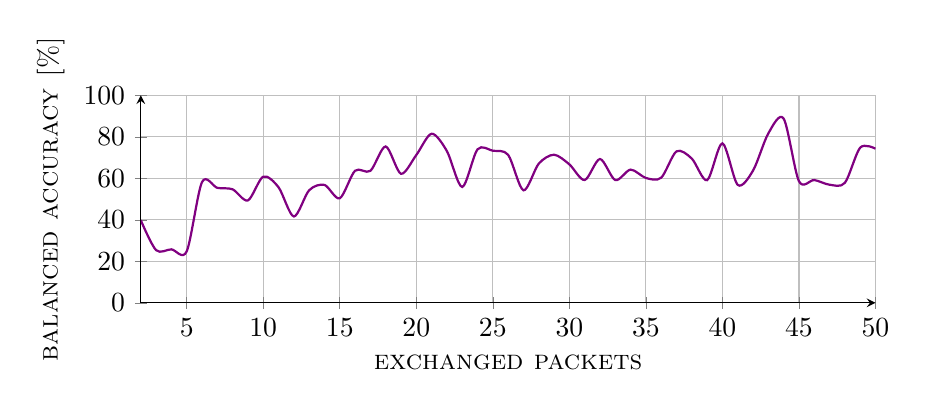
\begin{tikzpicture}
		\begin{axis}[xlabel=\textsc{exchanged packets}, ylabel=\textsc{balanced accuracy [$\%$]}, axis lines=left, grid=major, width=0.9\linewidth, height=12em, ymax=100, ymin=0]
			\addplot +[mark=none, Purple, thick, smooth] table {
				2.0 39.82014388489208
				3.0 25.37890352324433
				4.0 25.76909906125603
				5.0 24.788903279471537
				6.0 58.15627946087795
				7.0 55.39666559459041
				8.0 54.686574440762215
				9.0 49.34978492490254
				10.0 60.79292320332248
				11.0 55.67599410986571
				12.0 41.604812289832005
				13.0 54.23141903388486
				14.0 56.81959372696753
				15.0 50.36032460468392
				16.0 63.641997848681754
				17.0 63.583157700757944
				18.0 75.3311569794528
				19.0 62.184249722921834
				20.0 71.21251008420427
				21.0 81.47267040450839
				22.0 73.0903611677847
				23.0 55.83394591488062
				24.0 73.96223636921825
				25.0 73.27300330434355
				26.0 71.30163084042394
				27.0 54.20413661247863
				28.0 67.06335247629194
				29.0 71.35425758315066
				30.0 66.70200877553819
				31.0 59.16165928354725
				32.0 69.29730230055529
				33.0 59.147276334776336
				34.0 64.18491200130435
				35.0 60.15939307605974
				36.0 60.30143953710832
				37.0 72.99062049062049
				38.0 69.47896640968132
				39.0 59.10328254738712
				40.0 76.82906412188179
				41.0 56.82423906299674
				42.0 63.72685185185185
				43.0 81.66593419157977
				44.0 88.7585532746823
				45.0 58.59311740890688
				46.0 59.153591193821086
				47.0 56.90235690235691
				48.0 57.83272283272284
				49.0 74.77961432506888
				50.0 74.25760021522734
			};
		\end{axis}
	\end{tikzpicture}
	\caption{Balanced accuracy vs. exchange packets plot for the tool instance classifier based on extra-trees on the KTS.}
	\label{fig:packets_application_long_extra_trees}
\end{figure}
\begin{table}[H]
	\centering
	\begin{subtable}{.45\linewidth}
		\centering
	\begin{tabular}{ll}
		\toprule
		\textsc{inferred class} & \textsc{samples}\\
		\midrule
		chrome-48.0.2564.109 & 450\\
		chrome-68.0.3440.84 & 14\\
		curl-7.55.1 & 183\\
		curl-7.61.0 & 58\\
		edge-42.17134.1.0 & 573\\
		firefox-42.0 & 342\\
		firefox-62.0 & 1026\\
		goldeneye-2.1 & 472\\
		httrack-3.49.2 & 596\\
		hulk-1.0 & 2241\\
		rudy-1.0.0 & 22\\
		slowloris-0.1.4 & 2\\
		slowloris-0.1.5 & 23\\
		wget-1.11.4 & 49\\
		wget-1.19.5 & 260\\
		wpull-2.0.1 & 223\\
		\bottomrule
	\end{tabular}
	\caption{Classification of \textsc{firefox-68.0}.}
	\end{subtable}
	\begin{subtable}{.45\linewidth}
		\centering
	\begin{tabular}{ll}
		\toprule
		\textsc{inferred class} & \textsc{samples}\\
		\midrule
		chrome-48.0.2564.109 & 148\\
		chrome-68.0.3440.84 & 24\\
		curl-7.55.1 & 80\\
		curl-7.61.0 & 42\\
		edge-42.17134.1.0 & 217\\
		firefox-42.0 & 46\\
		firefox-62.0 & 156\\
		goldeneye-2.1 & 1039\\
		httrack-3.49.2 & 404\\
		hulk-1.0 & 22\\
		rudy-1.0.0 & 20\\
		slowloris-0.1.4 & 97\\
		slowloris-0.1.5 & 123\\
		wget-1.11.4 & 198\\
		wget-1.19.5 & 170\\
		wpull-2.0.1 & 879\\
		\bottomrule
	\end{tabular}
	\caption{Classification of \textsc{grabsite-2.1.16}.}
	\end{subtable}
	\begin{subtable}{.45\linewidth}
		\centering
	\begin{tabular}{ll}
		\toprule
		\textsc{inferred class} & \textsc{samples}\\
		\midrule
		chrome-48.0.2564.109 & 1913\\
		chrome-68.0.3440.84 & 1672\\
		curl-7.55.1 & 503\\
		curl-7.61.0 & 22\\
		edge-42.17134.1.0 & 432\\
		firefox-42.0 & 192\\
		firefox-62.0 & 220\\
		goldeneye-2.1 & 2978\\
		httrack-3.49.2 & 341\\
		hulk-1.0 & 41\\
		rudy-1.0.0 & 166\\
		slowloris-0.1.4 & 19\\
		slowloris-0.1.5 & 80\\
		wget-1.11.4 & 92\\
		wget-1.19.5 & 81\\
		wpull-2.0.1 & 198\\
		\bottomrule
	\end{tabular}
	\caption{Classification of \textsc{opera-62.0.3331.66}.}
	\end{subtable}
	\begin{subtable}{.45\linewidth}
		\centering
	\begin{tabular}{ll}
		\toprule
		\textsc{inferred class} & \textsc{samples}\\
		\midrule
		chrome-48.0.2564.109 & 271\\
		chrome-68.0.3440.84 & 214\\
		curl-7.55.1 & 6\\
		curl-7.61.0 & 19\\
		edge-42.17134.1.0 & 1473\\
		firefox-42.0 & 211\\
		firefox-62.0 & 581\\
		goldeneye-2.1 & 1965\\
		httrack-3.49.2 & 920\\
		hulk-1.0 & 32\\
		rudy-1.0.0 & 2674\\
		slowloris-0.1.4 & 160\\
		slowloris-0.1.5 & 1592\\
		wget-1.11.4 & 226\\
		wget-1.19.5 & 13\\
		wpull-2.0.1 & 638\\
		\bottomrule
	\end{tabular}
	\caption{Classification of \textsc{slowhttptest-1.6}.}
	\end{subtable}
	\caption{Classification of unknown tools for the tool instance classifier based on extra-trees.}
	\label{tab:unknown_application_long_extra_trees}
\end{table}
